\section*{Chapter 1}

\subsection*{Exercise 1.1}

\begin{enumerate}
    \item
    \begin{minipage}[t]{0.45\linewidth}
        $x = 2y^2$
    \end{minipage}
    \begin{minipage}[t]{0.45\linewidth}
        \begin{center}
            \tikzsetnextfilename{c01e01-01}%
            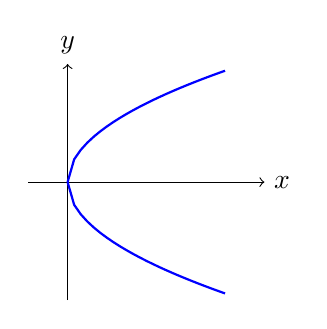
\begin{tikzpicture}[baseline=(current bounding box.west)]
                \draw[->] (-0.5, 0) -- (2.5, 0) node[right] {$x$};
                \draw[->] (0, -1.5) -- (0, 1.5) node[above] {$y$};

                \draw[thick,blue,domain=0:2] plot (\x, {sqrt(\x)});
                \draw[thick,blue,domain=0:2] plot (\x, {-sqrt(\x)});
            \end{tikzpicture}
        \end{center}
    \end{minipage}

    \item
    \begin{minipage}[t]{0.45\linewidth}
        $\begin{aligned}[t]
            \frac{x^2}{2} + \frac{y^2}{9}                                  & = 1 \\
            \left(\frac{x}{\sqrt{2}}\right)^2 + \left(\frac{y}{3}\right)^2 & = 1
        \end{aligned}$
    \end{minipage}
    \begin{minipage}[t]{0.45\linewidth}
        \begin{center}
            \tikzsetnextfilename{c01e01-02}%
            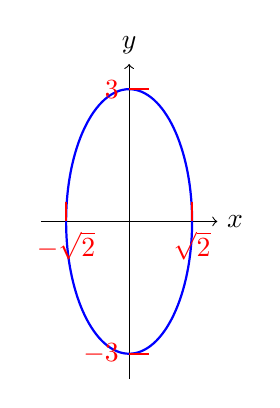
\begin{tikzpicture}[baseline=(current bounding box.west)]
                \draw[->] (-1.12, 0) -- (1.12, 0) node[right] {$x$};
                \draw[->] (0, -2) -- (0, 2) node[above] {$y$};

                \draw[thick,blue] (0, 0) ellipse (0.8cm and 1.68cm);

                \draw[thick,red] (0.8, 0.25) -- (0.8, 0) node[below,red] {$\sqrt{2}$};
                \draw[thick,red] (-0.8, 0.25) -- (-0.8, 0) node[below,red] {$-\sqrt{2}$};
                \draw[thick,red] (0.25, 1.68) -- (0, 1.68) node[left,red] {$3$};
                \draw[thick,red] (0.25, -1.68) -- (0, -1.68) node[left,red] {$-3$};
            \end{tikzpicture}
        \end{center}
    \end{minipage}

    \item
    \begin{minipage}[t]{0.45\linewidth}
        $\begin{aligned}[t]
            x^2 + 2y^2                                                     & = 4 \\
            \frac{x^2}{4} + \frac{2y^2}{4}                                 & = 1 \\
            \left(\frac{x}{2}\right)^2 + \left(\frac{y}{\sqrt{2}}\right)^2 & = 1
        \end{aligned}$
    \end{minipage}
    \begin{minipage}[t]{0.45\linewidth}
        \begin{center}
            % \tikzsetnextfilename{c01e01-03}%
            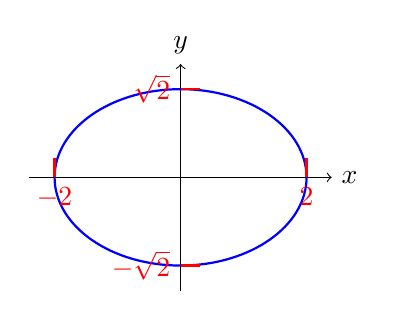
\begin{tikzpicture}[baseline=(current bounding box.north)]
                \draw[->] (-1.92, 0) -- (1.92, 0) node[right] {$x$};
                \draw[->] (0, -1.44) -- (0, 1.44) node[above] {$y$};

                \draw[thick,blue] (0, 0) ellipse (1.6cm and 1.12cm);

                \draw[thick,red] (1.6, 0.25) -- (1.6, 0) node[below,red] {$2$};
                \draw[thick,red] (-1.6, 0.25) -- (-1.6, 0) node[below,red] {$-2$};
                \draw[thick,red] (0.25, 1.12) -- (0, 1.12) node[left,red] {$\sqrt{2}$};
                \draw[thick,red] (0.25, -1.12) -- (0, -1.12) node[left,red] {$-\sqrt{2}$};
            \end{tikzpicture}
        \end{center}
    \end{minipage}

    \item
    \begin{minipage}[t]{0.45\linewidth}
        $\begin{aligned}[t]
            x^2 + 3y^2 + 2x - 12y + 10                                             & = 0 \\
            (x^2 + 2x + 1) + 3(y^2 - 4y + 4) - 3                                   & = 0 \\
            (x + 1)^2 + 3(y - 2)^2                                                 & = 3 \\
            \left(\frac{x + 1}{\sqrt{3}}\right)^2 + \left(\frac{y - 2}{1}\right)^2 & = 1
        \end{aligned}$

        Ellipse before the shift (in {\color{DarkGreen}green}): $$\left(\frac{x}{\sqrt{3}}\right)^2 + \left(\frac{y}{1}\right)^2 = 1$$

        Then, shift $1$ unit left and $2$ units up.
    \end{minipage}
    \begin{minipage}[t]{0.45\linewidth}
        \begin{center}
            \tikzsetnextfilename{c01e01-04}%
            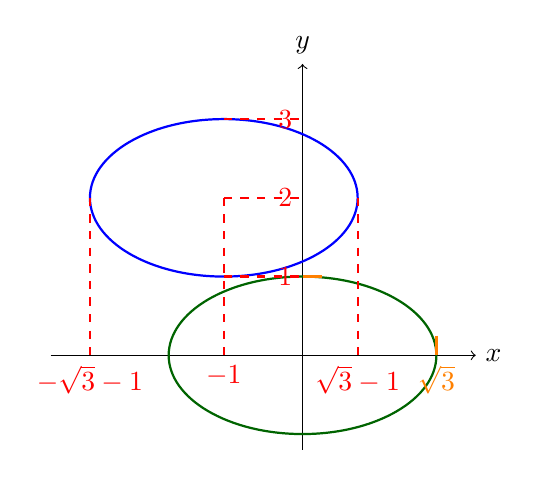
\begin{tikzpicture}[baseline=(current bounding box.north)]
                \draw[->] (-3.2, 0) -- (2.2, 0) node[right] {$x$};
                \draw[->] (0, -1.2) -- (0, 3.7) node[above] {$y$};

                \draw[thick,DarkGreen] (0, 0) ellipse (1.7cm and 1cm);
                \draw[thick,blue] (-1, 2) ellipse (1.7cm and 1cm);

                \draw[thick,orange] (1.7, 0.25) -- (1.7, 0) node[below] {$\sqrt{3}$};
                \draw[thick,orange] (0.25, 1) -- (0, 1) node[left,red] {$1$};

                \draw[thick,red,dashed] (0.7, 2) -- (0.7, 0) node[below] {$\sqrt{3} - 1$};
                \draw[thick,red,dashed] (-2.7, 2) -- (-2.7, 0) node[below] {$-\sqrt{3} - 1$};

                \draw[thick,red,dashed] (-1, 2) -- (0, 2) node[left] {$2$};
                \draw[thick,red,dashed] (-1, 2) -- (-1, 0) node[below] {$-1$};

                \draw[thick,red,dashed] (-1, 3) -- (0, 3) node[left] {$3$};
                \draw[thick,red,dashed] (-1, 1) -- (0, 1);
            \end{tikzpicture}
        \end{center}
    \end{minipage}

    \item
    \begin{minipage}[t]{0.45\linewidth}
        $y^2 - x^2 = 1$

        {~~~}

        If $y = 0$, then $-x^2 = 1$, not possible.

        Thus, the graph must not cross the horizontal axis, and the hyperbola opens \bred{up and down}.

        {~~~}

        If $x = 0$, then $y^2 = 1$, $y = \pm 1$.
    \end{minipage}
    \begin{minipage}[t]{0.45\linewidth}
        \begin{center}
            \tikzsetnextfilename{c01e01-05}%
            \begin{tikzpicture}[baseline=(current bounding box.north)]
                \draw[->] (-2.2, 0) -- (2.2, 0) node[right] {$x$};
                \draw[->] (0, -2.2) -- (0, 2.2) node[above] {$y$};

                \clip(-2, -2) rectangle (2, 2);

                \draw[thick,blue,rotate around={90:(0,0)},domain=-0.99:0.99] plot ({( 1+(\x)^2)/(1-(\x)^2)}, {  2 *(\x)/(1-(\x)^2)});
                \draw[thick,blue,rotate around={90:(0,0)},domain=-0.99:0.99] plot ({(-1-(\x)^2)/(1-(\x)^2)}, {(-2)*(\x)/(1-(\x)^2)});

                \draw[red] (0.25,-1) -- (0,-1) node[left] {$-1$};
                \draw[red] (0.25,1) -- (0,1) node[left] {$1$};
            \end{tikzpicture}
        \end{center}
    \end{minipage}

    \item
    \begin{minipage}[t]{0.45\linewidth}
        $\begin{aligned}[t]
            \frac{(x-2)^2}{4} - \frac{(y+2)^2}{9}                       & = 1 \\
            \left(\frac{x-2}{2}\right)^2 - \left(\frac{y+2}{3}\right)^2 & = 1
        \end{aligned}$

        {~~~}

        Hyperbola before the shift (in {\color{DarkGreen}green}): $$\left(\frac{x}{2}\right)^2 - \left(\frac{y}{3}\right)^2 = 1$$

        If $x = 0$, then $-y^2 = 1$, not possible.

        Thus, the graph must not cross the vertical axis, and the hyperbola opens \bred{left and right}.

        If $y = 0$, then $\left(\frac{x}{2}\right)^2 = 1$, $x = \pm 2$.
    \end{minipage}
    \begin{minipage}[t]{0.45\linewidth}
        \begin{center}
            \tikzsetnextfilename{c01e01-06}%
            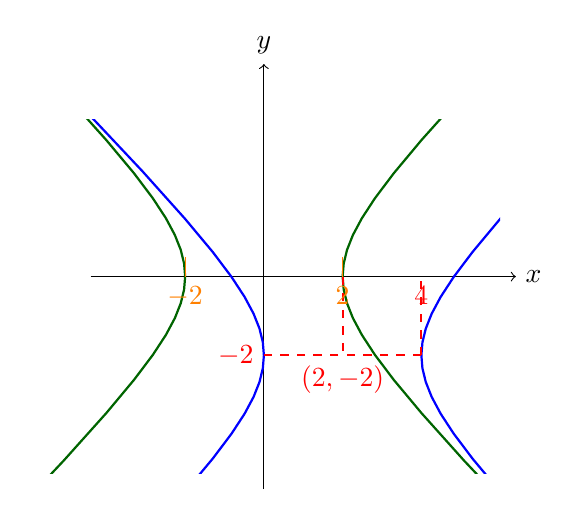
\begin{tikzpicture}[baseline=(current bounding box.north)]
                \draw[->] (-2.2, 0) -- (3.2, 0) node[right] {$x$};
                \draw[->] (0, -2.7) -- (0, 2.7) node[above] {$y$};

                \clip(-3, -2.5) rectangle (3, 2);

                \draw[thick,DarkGreen,domain=-0.99:0.99] plot ({( 1+(\x)^2)/(1-(\x)^2)}, {  2 *(\x)/(1-(\x)^2)});
                \draw[thick,DarkGreen,domain=-0.99:0.99] plot ({(-1-(\x)^2)/(1-(\x)^2)}, {(-2)*(\x)/(1-(\x)^2)});

                \draw[thick,blue,domain=-0.99:0.99] plot ({( 1+(\x)^2)/(1-(\x)^2) + 1}, {  2 *(\x)/(1-(\x)^2) - 1});
                \draw[thick,blue,domain=-0.99:0.99] plot ({(-1-(\x)^2)/(1-(\x)^2) + 1}, {(-2)*(\x)/(1-(\x)^2) - 1});

                \draw[thick,red,dashed] (2,-1) -- (0,-1) node[left] {$-2$};
                \draw[thick,red,dashed] (2,-1) -- (2,0) node[below] {$4$};
                \draw[thick,red,dashed] (1,0) -- (1,-1) node[below] {$(2,-2)$};

                \draw[orange] (-1,0.25) -- (-1,0) node[below] {$-2$};
                \draw[orange] (1,0.25) -- (1,0) node[below] {$2$};
            \end{tikzpicture}
        \end{center}
    \end{minipage}
\end{enumerate}

\subsection*{Exercise 1.2}

\begin{enumerate}
    \item
    \begin{minipage}[t]{0.25\linewidth}
        $\begin{aligned}[t]
            x^2 + y^2 & = 1 \\
            r^2       & = 1 \\
            r         & = 1
        \end{aligned}$
    \end{minipage}
    \begin{minipage}[c]{0.2\linewidth}
        \begin{center}
            \begin{tikzpicture}
                \draw[->] (-1.2, 0) -- (1.2, 0) node[right] {$r_{(y)}$};
                \draw[->] (0, -1.2) -- (0, 1.2) node[above] {$z$};

                \draw[thick,blue,domain=-1:1] plot (1, \x) node[left,red] {$r = 1$};
            \end{tikzpicture}
        \end{center}
    \end{minipage}
    \begin{minipage}[c]{0.5\linewidth}
        \begin{center} \includegraphics[width=0.9\linewidth]{Plots/e_1_2/1.png} \end{center}
    \end{minipage}

    \item
    \begin{minipage}[t]{0.25\linewidth}
        $\begin{aligned}[t]
            z & = x^2 + y^2 \\
            z & = r^2
        \end{aligned}$
    \end{minipage}
    \begin{minipage}[c]{0.2\linewidth}
        \begin{center}
            \begin{tikzpicture}
                \draw[->] (-1.2, 0) -- (1.2, 0) node[right] {$r_{(y)}$};
                \draw[->] (0, -0.7) -- (0, 1.7) node[above] {$z$};

                \draw[thick,blue,domain=0:1.25] plot (\x, {(\x)^2}) node[above,red] {$z = r^2$};
            \end{tikzpicture}
        \end{center}
    \end{minipage}
    \begin{minipage}[c]{0.5\linewidth}
        \begin{center} \includegraphics[width=0.9\linewidth]{Plots/e_1_2/2.png} \end{center}
    \end{minipage}

    \item
    \begin{minipage}[t]{0.25\linewidth}
        $\begin{aligned}[t]
            z^2 & = x^2 + y^2 \\
            z^2 & = r^2       \\
            z   & = \pm r
        \end{aligned}$
    \end{minipage}
    \begin{minipage}[c]{0.2\linewidth}
        \begin{center}
            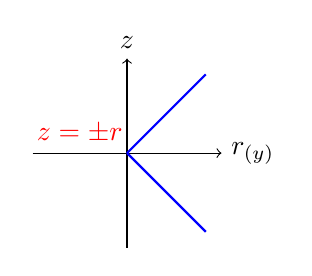
\begin{tikzpicture}
                \draw[->] (-1.2, 0) -- (1.2, 0) node[right] {$r_{(y)}$};
                \draw[->] (0, -1.2) -- (0, 1.2) node[above] {$z$};

                \draw[thick,blue,domain=0:1] plot (\x, {\x});
                \draw[thick,blue,domain=0:1] plot (\x, {-\x});

                \node[red] at (-0.6,0.25) {$z = \pm r$};
            \end{tikzpicture}
        \end{center}
    \end{minipage}
    \begin{minipage}[c]{0.5\linewidth}
        \begin{center} \includegraphics[width=0.9\linewidth]{Plots/e_1_2/3.png} \end{center}
    \end{minipage}

    \item
    \begin{minipage}[t]{0.25\linewidth}
        $\begin{aligned}[t]
            x^2 + y^2 + \frac{z^2}{4}                               & = 1 \\
            r^2 + \frac{z^2}{4}                                     & = 1 \\
            \left(\frac{r}{1}\right)^2 + \left(\frac{z}{2}\right)^2 & = 1
        \end{aligned}$
    \end{minipage}
    \begin{minipage}[c]{0.2\linewidth}
        \begin{center}
            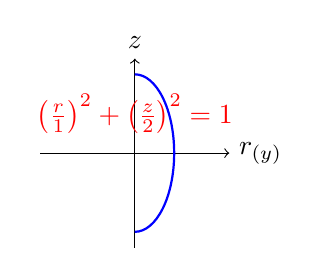
\begin{tikzpicture}
                \draw[->] (-1.2, 0) -- (1.2, 0) node[right] {$r_{(y)}$};
                \draw[->] (0, -1.2) -- (0, 1.2) node[above] {$z$};

                \draw[thick,blue] (0,1) arc (90:-90:0.5cm and 1cm);

                \node[red] at (0,0.5) {$\left(\frac{r}{1}\right)^2 + \left(\frac{z}{2}\right)^2 = 1$};
            \end{tikzpicture}
        \end{center}
    \end{minipage}
    \begin{minipage}[c]{0.5\linewidth}
        \begin{center} \includegraphics[width=0.9\linewidth]{Plots/e_1_2/4.png} \end{center}
    \end{minipage}

    \item
    \begin{minipage}[t]{0.25\linewidth}
        $\begin{aligned}[t]
            z & = \left(\sqrt{x^2 + y^2} - 1\right)^2 \\
            z & = (r - 1)^2
        \end{aligned}$
    \end{minipage}
    \begin{minipage}[c]{0.2\linewidth}
        \begin{center}
            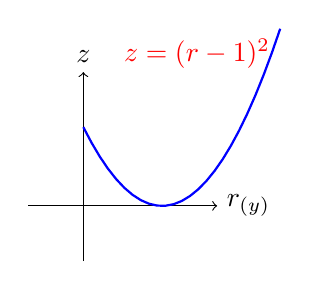
\begin{tikzpicture}
                \draw[->] (-0.7, 0) -- (1.7, 0) node[right] {$r_{(y)}$};
                \draw[->] (0, -0.7) -- (0, 1.7) node[above] {$z$};

                \draw[thick,blue,domain=0:2.5] plot (\x, {(\x - 1)^2}) node[below left,red] {$z = (r - 1)^2$};
            \end{tikzpicture}
        \end{center}
    \end{minipage}
    \begin{minipage}[c]{0.5\linewidth}
        \begin{center} \includegraphics[width=0.9\linewidth]{Plots/e_1_2/5.png} \end{center}
    \end{minipage}

    \item
    \begin{minipage}[t]{0.25\linewidth}
        $\begin{aligned}[t]
            x^2 + y^2 + z^2    & = 2z \\
            r^2 + z^2 - 2z + 1 & = 1  \\
            r^2 + (z - 1)^2    & = 1
        \end{aligned}$
    \end{minipage}
    \begin{minipage}[c]{0.2\linewidth}
        \begin{center}
            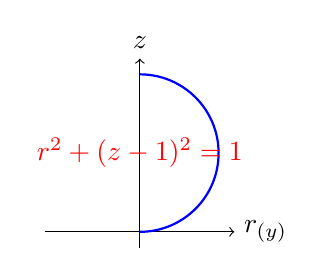
\begin{tikzpicture}
                \draw[->] (-1.2, 0) -- (1.2, 0) node[right] {$r_{(y)}$};
                \draw[->] (0, -0.2) -- (0, 2.2) node[above] {$z$};

                \draw[thick,blue] (0,2) arc (90:-90:1cm and 1cm);

                \node[red] at (0,1) {$r^2 + (z - 1)^2 = 1$};
            \end{tikzpicture}
        \end{center}
    \end{minipage}
    \begin{minipage}[c]{0.5\linewidth}
        \begin{center} \includegraphics[width=0.9\linewidth]{Plots/e_1_2/6.png} \end{center}
    \end{minipage}
\end{enumerate}